The individual particles have to be identified end segmented from the background. These operations are performed on the enhanced intensity matrix. If the user opted to use back lit and bright field matrices, the enhanced intensity matrices where calculated from the back lit intensity matrices. Otherwise the bright field intensity matrices are used.

\paragraph{Segmentation}\index{Segmentation}
The images are segmented by calculating a threshold value\index{Threshold}. This value is determined by using the Otsu\index{Otsu's method} threshold. \citeauthor{Xu2011956} \cite{Xu2011956} describe that the Otsu threshold is equal to the average of the mean levels of two classes partitioned by this threshold. This threshold value can be iteratively determined.

\begin{sBox}
	Let $\vec{h}$ be a vector of dimension $256$ which represent a count of values in the enhanced intensity matrix $\mat{I} \subset \mathbb{Z}^n \rightarrow \{0, 255\}$ with dimensions $m \times n$
	\begin{equation}\label{OtsuMethodEq}
		\frac{1}{t_o}\sum\limits_{i=1}^{t_o} \vec{h}_i = t_o - \frac{1}{256 - t_o}\sum\limits_{i=t_o}^{256} \vec{h}_i
	\end{equation}
\end{sBox}

In order to get more control over the segmentation process, the normal Otsu's method, as shown above is altered. A user now has the option to choose whether bright or dark object are segmented and how much the intensity values may deviation from the mean value. This mean value is either the left or right hand side of the equation \ref{OtsuMethodEq} modified with a scaling factor and the standard deviation, as shown in equation \ref{darkObjEq} and \ref{brightObjEq}.
\begin{sBox}
	Let $ t_o \subset \mathbb{Z}^n \rightarrow \{0\leq t \leq 255\}$ be the threshold value obtained with the iteration algorithm used to solve equation \ref{OtsuMethodEq}, $ \alpha $ be the a multiplication factor given by the user and let $\vec{h} \subset \mathbb{Z}^n$ be a vector of dimension $256$ which represent a count of values in the enhanced intensity matrix $\mat{I} \subset \mathbb{Z}^n \rightarrow \{0, 255\}$ with dimensions $m \times n$\\	
	If dark objects are to be obtained
	\begin{equation}\label{darkObjEq}
		t = \frac{1}{t_o}\mu + \frac{1}{2}\alpha\sigma {\rm \ \ where\ \ }\sigma = \sqrt{\frac{1}{t_o} \sum\limits_{i=1}^t (\vec{h}_i - \mu)^2}, {\rm \ \ and\ \ } \mu = \frac{1}{t_o} \sum\limits_{i=1}^t \vec{h}_i
	\end{equation}
	 else
	 \begin{equation}\label{brightObjEq}
	 	t = \frac{1}{t_o}\mu - \frac{1}{2}\alpha\sigma {\rm \ \ where\ \ }\sigma = \sqrt{\frac{1}{256 - t_o} \sum\limits_{i=t}^{256} (\vec{h}_i - \mu)^2}, {\rm \ \ and\ \ } \mu = \frac{1}{256 - t_o} \sum\limits_{i=t}^{256} \vec{h}_i
	 \end{equation} 
\end{sBox}

\paragraph{Binary Image}\index{Binary Image}\index{BW}\label{binaryImage} The binary image is calculated by using the previous obtained threshold value as illustrated in equation \ref{BWeq}.
\begin{sBox}
	Let $\mat{B} \subset \mathbb{Z}^n \rightarrow \{0, 1\}$ and $\mat{I} \subset \mathbb{Z}^n \rightarrow \{0, 255\}$ both with dimensions $ m \times n $ and let $t \subset \mathbb{Z}^n \rightarrow \{0\leq t \leq 255\}$
	\begin{equation}\label{BWeq}
		\mat{B} = \floor*{\frac{\mat{I}}{t}}
	\end{equation}
\end{sBox}

\paragraph{Labeled blobs}\index{Blobs}\index{Labeled blobs}
\begin{wrapfigure}{r}{0.50\textwidth}
	\begin{center}
		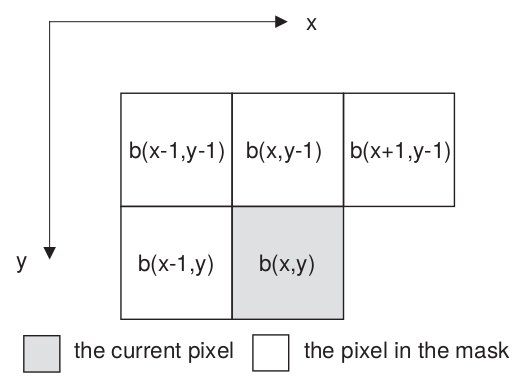
\includegraphics[width=0.495\textwidth]{nBors.png}
	\end{center}
	\caption{Neighboring elements Source: \cite{he_fast_2009}}
	\label{fig:Neighboring_elements}
\end{wrapfigure}
If the threshold value was correctly ascertained then the binary image will consist of zeros and ones. In this matrix the particles are represented by islands of connected elements with a designated value of one in an ocean of zeros. The individual particles, which are dubbed "blobs" will be identified with a two-pass connected-component labeling algorithm. This algorithm passes each element in a binary image in a consecutive manner. When the current element belongs to a particle, it will check if previous processed neighboring pixels belong to an previously labeled blob. If this is not the case it will assign a new label value to the current element. If it finds that one of the neighbors belong to one or more blobs, it assigns the lowest value and writes the other value to a queue. So it knows which labels are interlinked with each other.

\begin{figure}[h]
	\centering
	\begin{tikzpicture}[->,>=stealth', shorten >=1pt,auto,node distance=2cm, thick,main node/.style={circle,fill=ocre!20,draw}]
	\node[main node] (1) {1};
	\node[main node] (2) [below of=1] {2};
	\node[main node] (3) [right of=2] {3};
	\node[main node] (4) [right of=3] {5};
	\node[main node] (5) [below of=3] {6};
	\node[main node] (6) [right of=5] {9};
	\node[main node] (7) [below of=5] {10};
	\node[main node] (8) [below of=7] {12};
	
	
	\path[-]
	(1) edge node {} (2)
	(2) edge node {} (5)
	(3) edge node {} (5)
	(5) edge node {} (7)
	(4) edge node {} (6)
	(6) edge node {} (7)
	(7) edge node {} (8);
	\end{tikzpicture}
	\caption{Connected Queue}
	\label{ConnQue}
\end{figure}

In order to determine the lowest value of the connected component, there are graphs matrices generated, see figure \ref{ConnQue}. Each branch on these trees are followed till the lowest value is ascertained. All the leafs on the tree are then set to this value. These values are placed in a Look-Up-Table\index{Look-Up-Table}. With the second loop through the previously labeled image each value is replaced by looking up the lowest value in LUT.  
\begin{remark}
	A Look-Up-Table (LUT) is an array where a new value can be obtained with a simple array indexing operation. This is a very effective operation since looking up a value in memory cost less machine instructions then perform computation on each matrix element. A LUT consist of 256 elements for a unsigned byte, while a image matrix has roughly 5 million elements. 
\end{remark}